% HISTÓRICA: de antes de las ranuras de medición, que retiraron esta decisión
% (ver docs/mca/vista_general_mca.md, Decisiones retiradas).
% D6 por dentro: la lógica de `armed` en mca_window.
% Cada modo calcula el valor siguiente; después, en el orden del always (lo
% último gana), abrir lo consume y run = 0 en reposo lo baja. Lo que sale es UN
% flip-flop, y tres cosas lo leen: la apertura, el casillero t_rearm y la
% atribución de arribos.
% Fuente: modulos/mca/rtl/mca_window.sv ("re-armado: por NIVEL o por CONTADOR").
% Compilar:   pdflatex d06_rearmado_logica.tex && pdftocairo -svg d06_rearmado_logica.pdf d06_rearmado_logica.svg
\documentclass[border=0pt,tikz]{standalone}
\usepackage[utf8]{inputenc}
\usepackage[T1]{fontenc}
\usepackage{lmodern}
\usepackage[none]{hyphenat}
% Estilo común de las figuras TikZ (panoramas y diagramas de bloques).
%
% Cada figura lo incluye con \input{../../figuras/estilo_tikz.tex} (las figuras
% viven en docs/<módulo>/figuras/). Un solo lugar para la paleta, los estilos de
% bloque y el formato de los parámetros: si cambia algo acá, cambia en todas.
%
% La paleta es la misma de docs/figuras/estilo_svg.py y de PALETA en
% modulos/mk/datasheet.py; si se toca un color, se toca en los tres.
%
% Requiere: \usepackage{tikz} (lo da la clase standalone con la opción tikz).

\usetikzlibrary{arrows.meta,positioning,calc,fit,backgrounds,shapes.multipart,
                decorations.markings,shadows}

% ---------------------------------------------------------------- colores ---
\definecolor{azul}{RGB}{108,172,228}      % acondicionamiento
\definecolor{verde}{RGB}{110,214,142}     % captura / histogramas en BRAM
\definecolor{amarillo}{RGB}{252,232,160}  % trigger
\definecolor{naranja}{RGB}{252,206,160}   % camino a DDR
\definecolor{grisr}{RGB}{226,226,226}     % compartido / infraestructura
\definecolor{rojo}{RGB}{240,128,128}      % bus del sistema

% ---------------------------------------------------------------- estilos ---
\tikzset{
  >={Stealth[length=2.4mm,width=1.8mm]},
  % fondo blanco siempre: el SVG se ve igual en modo claro y oscuro
  fondo/.style   = {show background rectangle, inner frame sep=8pt,
                    background rectangle/.style={fill=white, draw=none}},
  bloque/.style  = {draw=black, line width=0.6pt, rounded corners=2pt,
                    align=center, text width=2.2cm, minimum height=1.15cm,
                    inner sep=2pt, font=\scriptsize, fill=#1},
  datos/.style   = {bloque=azul!35},
  trig/.style    = {bloque=amarillo},
  captura/.style = {bloque=verde!55},
  ddr/.style     = {bloque=naranja!70},
  comp/.style    = {bloque=grisr},
  bus/.style     = {bloque=rojo!45},
  % lógica escrita dentro del módulo, sin submódulo propio
  etapa/.style   = {bloque=#1, line width=0.5pt},
  etapa/.default = verde!20,
  % lo que el bitstream no trae (atado a cero, stub, salida muda)
  mudo/.style    = {bloque=white, draw=black!45, dashed, text=black!55},
  %
  % BLOQUE CON PARÁMETROS, en el formato del datasheet: el encabezado lleva el
  % nombre y los parámetros con que lo instancia el padre (NOMBRE=valor, en
  % monoespaciada, uno por línea); el cuerpo, más claro, lo que hace.
  %   \node[datos, param={azul!35}{azul!12}] {\blk{nombre}{} \prm{A=1\\B=2}
  %                                            \nodepart{two} función};
  param/.style 2 args = {rectangle split, rectangle split parts=2,
                         rectangle split part fill={#1, #2}},
  %
  flujo/.style   = {->, line width=0.8pt},
  ctrl/.style    = {->, line width=0.6pt, black!65},
  % la línea que pasa por encima en un cruce: un halo blanco la separa
  cruce/.style   = {preaction={draw=white, line width=3.4pt, -}},
  % marca de ancho de bus: barra oblicua a mitad de la flecha, con el número
  % encima. \draw[flujo, ancho=14] ...; para otra posición, ancho en=0.3.
  ancho/.style   = {decoration={markings, mark=at position \anchopos with {
                      \draw[line width=0.6pt, -] (-0.1,-0.14) -- (0.1,0.14);
                      \node[font=\scriptsize, above=1.5pt] {#1};}},
                    postaction={decorate}},
  % la misma marca en una flecha vertical: el número va a la derecha
  anchov/.style  = {decoration={markings, mark=at position \anchopos with {
                      \draw[line width=0.6pt, -] (-0.14,-0.1) -- (0.14,0.1);
                      \node[font=\scriptsize, right=3pt] {#1};}},
                    postaction={decorate}},
  ancho en/.code = {\def\anchopos{#1}},
  sen/.style     = {font=\scriptsize\ttfamily, inner sep=1.5pt},
  nodo/.style    = {font=\tiny\ttfamily, inner sep=1pt, black!75},
  pin/.style     = {font=\scriptsize, align=center, inner sep=1pt},
  grupo/.style   = {draw=black!55, dashed, line width=0.7pt, rounded corners=4pt},
  canal/.style   = {grupo},
  contenedor/.style = {draw=black!80, line width=1.0pt, rounded corners=6pt},
  % marca numerada: cada número es una fila de la tabla del documento
  marca/.style   = {circle, fill=black, text=white, font=\scriptsize\bfseries,
                    inner sep=0pt, minimum size=4.3mm},
  %
  % DECISIONES (docs/mca/vista_general_mca.md). Cada opción es un bloque, todas
  % entran a un mux (\muxdec, abajo) y el registro que elige entra por abajo.
  % la opción que trae el reset (el comportamiento histórico): borde doble
  defecto/.style = {double=white, double distance=0.8pt, line width=0.45pt},
  % rótulo de la decisión, el mismo Dn del panorama y del documento
  decision/.style = {circle, fill=black, text=white, font=\small\bfseries,
                     inner sep=0pt, minimum size=7mm},
  %
  % LÓGICA (docs/mca/figuras/contabilidad/ y los detalles de las decisiones)
  % registro: caja gris con el triángulo de reloj en el borde de abajo
  registro/.style = {draw=black, line width=0.6pt, fill=grisr, align=center,
                     font=\scriptsize, inner sep=2pt, minimum width=#1,
                     minimum height=0.85cm,
                     path picture={\draw[line width=0.5pt]
                       ([xshift=-1.1mm]path picture bounding box.south) --
                       ([yshift=1.6mm]path picture bounding box.south) --
                       ([xshift=1.1mm]path picture bounding box.south);}},
  registro/.default = 0.8cm,
  % condición de una cadena if / else-if: "sí" sale a la derecha, "no" abajo
  pregunta/.style = {draw=black, line width=0.5pt, rounded corners=7pt,
                     fill=white, font=\scriptsize\ttfamily, align=center,
                     inner sep=2.5pt, minimum height=0.62cm, text width=#1},
  pregunta/.default = 1.9cm,
  si/.style      = {font=\tiny, inner sep=1pt, above, pos=0.12},
  no/.style      = {font=\tiny, inner sep=1pt, left, pos=0.45},
  %
  titulo/.style  = {anchor=north west, font=\small, inner sep=4pt, align=left},
  rotulo/.style  = {anchor=north west, font=\scriptsize\itshape, black!70,
                    inner sep=2pt, align=left},
}

% submódulo: nombre en monoespaciada; lógica propia: nombre en romana
\newcommand{\blk}[2]{{\ttfamily\bfseries #1}\\[1pt]#2}
\newcommand{\etq}[2]{{\bfseries #1}\\[1pt]#2}
\newcommand{\punto}[1]{\fill (#1) circle (1.3pt);}

% Parámetros en el formato del datasheet: NOMBRE=valor en monoespaciada, una
% entrada por celda, hasta cuatro columnas. Una columna: \prm{A=1\\B=2};
% dos: \prm{A=1 & B=2\\C=3}.
\newcommand{\prm}[1]{{\ttfamily\fontsize{5.6}{6.6}\selectfont
  \begin{tabular}{@{}l@{\hspace{7pt}}l@{\hspace{7pt}}l@{\hspace{7pt}}l@{}}#1\end{tabular}}}

\def\anchopos{0.5}

% Mux de una decisión: trapecio con el lado ancho (las entradas) a la izquierda.
% #1 = nombre, #2 = centro, #3 = alto en cm. Deja tres coordenadas:
%   (#1-in)  centro del lado de entradas: las flechas llegan a (#1-in |- opcion.east)
%   (#1-out) la salida
%   (#1-sel) mitad del lado de abajo: por ahí entra el registro que elige
% El rótulo de adentro es opcional: \muxdec{m}{(4,0)}{3.6} y después
% \node[...] at (m) {...}.
\newcommand{\muxdec}[3]{%
  \path #2 coordinate (#1);
  \draw[line width=0.6pt, fill=grisr]
    ($(#1)+(-0.45,{#3/2})$) -- ($(#1)+(0.45,{#3/2-0.35})$) --
    ($(#1)+(0.45,{-#3/2+0.35})$) -- ($(#1)+(-0.45,{-#3/2})$) -- cycle;
  \coordinate (#1-in)  at ($(#1)+(-0.45,0)$);
  \coordinate (#1-out) at ($(#1)+(0.45,0)$);
  \coordinate (#1-sel) at ($(#1)+(0,{-#3/2+0.175})$);}

% El mismo mux rotado 90 grados, para un flujo de arriba hacia abajo: entradas
% por el lado ancho de arriba, salida abajo y el registro que elige por la
% izquierda. #1 = nombre, #2 = centro, #3 = ancho en cm. Deja (#1-in) centro del
% lado de entradas, (#1-out) la salida y (#1-sel) mitad del lado izquierdo.
\newcommand{\muxdecv}[3]{%
  \path #2 coordinate (#1);
  \draw[line width=0.6pt, fill=grisr]
    ($(#1)+({-#3/2},0.45)$) -- ($(#1)+({#3/2},0.45)$) --
    ($(#1)+({#3/2-0.35},-0.45)$) -- ($(#1)+({-#3/2+0.35},-0.45)$) -- cycle;
  \coordinate (#1-in)  at ($(#1)+(0,0.45)$);
  \coordinate (#1-out) at ($(#1)+(0,-0.45)$);
  \coordinate (#1-sel) at ($(#1)+({-#3/2+0.175},0)$);}

% Leyenda de colores + nota. #1 = posición, #2 = color/texto, #3 = nota.
\newcommand{\leyenda}[3]{%
  \begin{scope}[shift={(#1)}, every node/.style={font=\scriptsize}]
    \coordinate (t0) at (-0.5,0);
    \foreach \c/\t [count=\i] in {#2} {
      \pgfmathtruncatemacro\j{\i-1}
      \node[draw, fill=\c, minimum width=4mm, minimum height=3mm, inner sep=0pt,
            right=5mm of t\j.east, anchor=west] (l\i) {};
      \node[right=1.5mm of l\i] (t\i) {\t};
    }
    \node[anchor=north west, black!70, text width=19cm, align=left]
      at (-0.05,-0.3) {#3};
  \end{scope}}

% Lo que dicen los parámetros, para la nota de la leyenda
\newcommand{\notaparam}{\texttt{NOMBRE=valor}: parámetros con que el padre
  instancia el bloque (se omiten los que sólo pasan el del padre sin cambio).}

\tikzset{lee/.style = {etapa, text width=2.75cm, align=left}}

\begin{document}
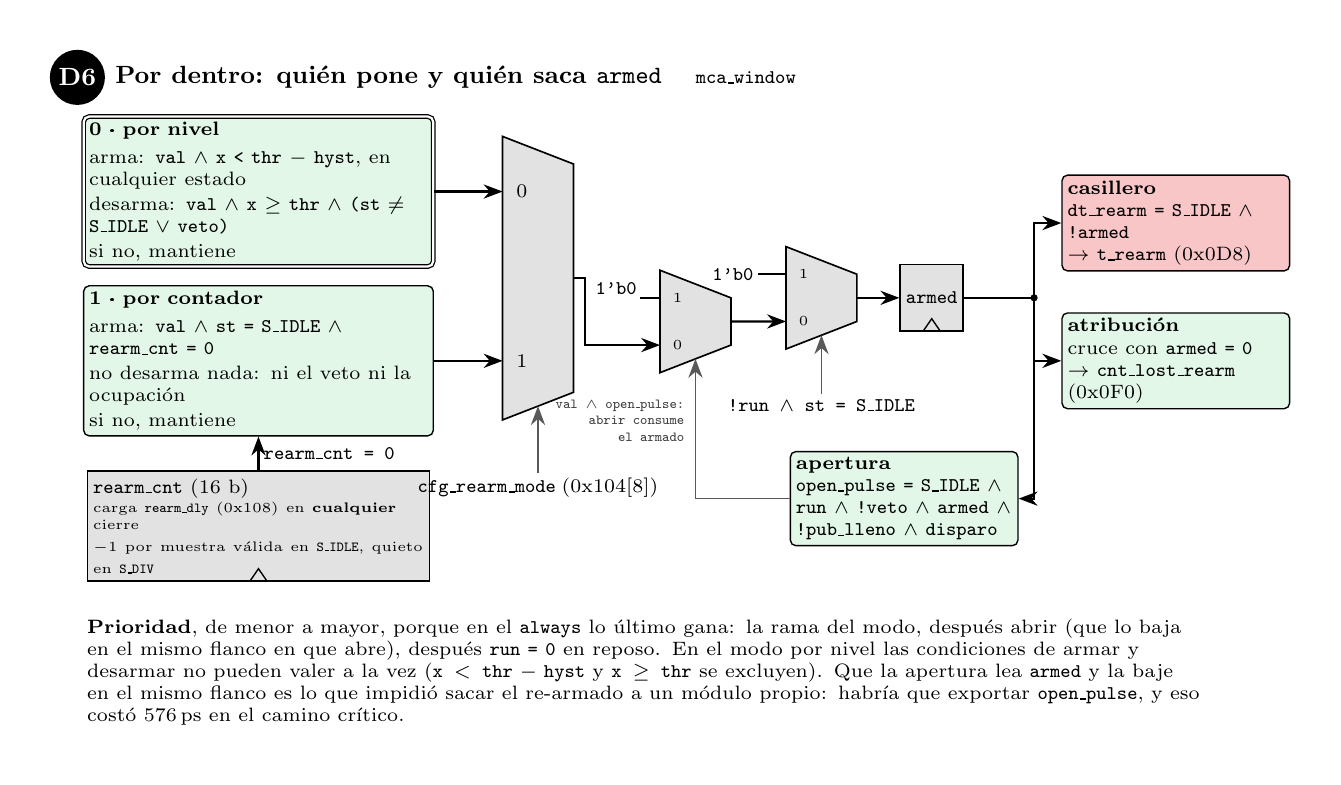
\begin{tikzpicture}[fondo]

\node[decision] (d) at (-0.9,2.75) {D6};
\node[anchor=west, font=\small] at (d.east)
  {\textbf{Por dentro: quién pone y quién saca \texttt{armed}} \quad
   {\scriptsize\ttfamily mca\_window}};

% ============================================== el valor siguiente, por modo
\node[etapa, defecto, text width=4.3cm, align=left] (o0) at (1.4,1.3)
  {\textbf{0 · por nivel}\\[2pt]
   arma: \texttt{val $\wedge$ x < thr $-$ hyst}, en cualquier estado\\[1pt]
   desarma: \texttt{val $\wedge$ x $\ge$ thr $\wedge$ (st $\ne$ S\_IDLE $\vee$ veto)}\\[1pt]
   si no, mantiene};
\node[etapa, text width=4.3cm, align=left] (o1) at (1.4,-0.85)
  {\textbf{1 · por contador}\\[2pt]
   arma: \texttt{val $\wedge$ st = S\_IDLE $\wedge$ rearm\_cnt = 0}\\[1pt]
   no desarma nada: ni el veto ni la ocupación\\[1pt]
   si no, mantiene};
\node[registro, text width=4.2cm, align=left, minimum height=1.4cm] (cnt) at (1.4,-2.95)
  {\texttt{rearm\_cnt} (16 b)\\[1pt]
   \tiny carga \texttt{rearm\_dly} (0x108) en \textbf{cualquier} cierre\\
   \tiny $-1$ por muestra válida en \texttt{S\_IDLE}, quieto en \texttt{S\_DIV}};
\draw[flujo] (cnt.north) -- node[sen, right] {rearm\_cnt = 0} (o1.south);

\muxdec{m}{(4.95,0.2)}{3.6}
\draw[flujo] (o0.east) -- (m-in |- o0.east);
\draw[flujo] (o1.east) -- (m-in |- o1.east);
\node[font=\scriptsize, anchor=west] at ($(m-in |- o0.east)+(0.05,0)$) {0};
\node[font=\scriptsize, anchor=west] at ($(m-in |- o1.east)+(0.05,0)$) {1};
\draw[ctrl] ($(m-sel)+(0,-0.85)$) node[below, sen, black] {cfg\_rearm\_mode\;\normalfont(0x104[8])}
  -- (m-sel);

% ======================================= lo que gana después, en ese orden
\muxdec{f1}{(6.95,-0.35)}{1.3}
\draw[flujo] (m-out) -- (5.55,0.2) |- ($(f1-in)+(0,-0.3)$);
\draw[line width=0.6pt] ($(f1-in)+(0,0.3)$) -- ++(-0.25,0) node[sen, above left, inner sep=1pt] {1'b0};
\node[font=\tiny, anchor=west] at ($(f1-in)+(0.04,-0.3)$) {0};
\node[font=\tiny, anchor=west] at ($(f1-in)+(0.04,0.3)$) {1};

\muxdec{f2}{(8.55,-0.05)}{1.3}
\draw[flujo] (f1-out) -- ($(f2-in)+(0,-0.3)$);
\draw[line width=0.6pt] ($(f2-in)+(0,0.3)$) -- ++(-0.35,0) node[sen, left] {1'b0};
\node[font=\tiny, anchor=west] at ($(f2-in)+(0.04,-0.3)$) {0};
\node[font=\tiny, anchor=west] at ($(f2-in)+(0.04,0.3)$) {1};
\draw[ctrl] ($(f2-sel)+(0,-0.75)$) node[below, sen, black, align=center]
  {!run $\wedge$ st = S\_IDLE} -- (f2-sel);

\node[registro] (ff) at (9.95,-0.05) {\texttt{armed}};
\draw[flujo] (f2-out) -- (ff.west);

% ================================================= quién lee el flip-flop
\node[lee] (ap) at (9.6,-2.6)
  {\textbf{apertura}\\ \texttt{open\_pulse = S\_IDLE $\wedge$ run $\wedge$ !veto $\wedge$ armed $\wedge$ !pub\_lleno $\wedge$ disparo}};
\node[lee, fill=rojo!45] (tr) at (13.05,0.9)
  {\textbf{casillero}\\ \texttt{dt\_rearm = S\_IDLE $\wedge$ !armed}\\ $\to$ \texttt{t\_rearm} (0x0D8)};
\node[lee] (at) at (13.05,-0.85)
  {\textbf{atribución}\\ cruce con \texttt{armed = 0}\\ $\to$ \texttt{cnt\_lost\_rearm} (0x0F0)};
\draw[line width=0.8pt] (ff.east) -- (11.25,-0.05);
\punto{11.25,-0.05}
\draw[flujo] (11.25,-0.05) |- (tr.west);
\draw[flujo] (11.25,-0.05) |- (at.west);
\draw[flujo] (11.25,-0.05) |- (ap.east);

% abrir consume el armado: la apertura vuelve sobre el primer forzado
\draw[ctrl] (ap.west) -| (f1-sel);
\node[nodo, anchor=north east, align=right] at (6.85,-1.3) {\texttt{val $\wedge$ open\_pulse}:\\ abrir consume\\ el armado};

% ===================================================================== nota
\node[anchor=north west, font=\scriptsize, align=left, text width=14.2cm] at (-0.9,-4.0)
  {\textbf{Prioridad}, de menor a mayor, porque en el \texttt{always} lo último gana:
   la rama del modo, después abrir (que lo baja en el mismo flanco en que abre),
   después \texttt{run = 0} en reposo. En el modo por nivel las condiciones de armar
   y desarmar no pueden valer a la vez ($\texttt{x} < \texttt{thr} - \texttt{hyst}$ y
   $\texttt{x} \ge \texttt{thr}$ se excluyen). Que la apertura lea \texttt{armed} y la
   baje en el mismo flanco es lo que impidió sacar el re-armado a un módulo propio:
   habría que exportar \texttt{open\_pulse}, y eso costó 576\,ps en el camino crítico.};

\end{tikzpicture}
\end{document}
